% beamer configuration
\mode<all>
\setbeamertemplate{itemize items}[default]
\setbeamertemplate{navigation symbols}{}
\setbeamertemplate{block begin}{}
\setbeamertemplate{headline}{}
\setbeamertemplate{footline}{}

% \testimonyWithContent: create a new testimony based on austama template.
%
% @arg1: Firstname Lastname
% @arg2: Location
% @arg3: Age
% @arg4: Vaccine type
% @arg5: Injection dates
% @arg6: Adverse Drug Reaction
% @arg7: Source URL
% @arg8: Testimony
\newcommand{\testimonyWithContent}[8]{
  \begin{frame}{}
    \vfill
    \begin{center}
      \textbf{\VERYHuge {#1} } \\
      \vspace{0.25cm}
      \Large {#2} \\
      \vspace{0.25cm}
      \begin{multicols}{2}
        \begin{minipage}{\linewidth}
        \begin{FlushLeft}
          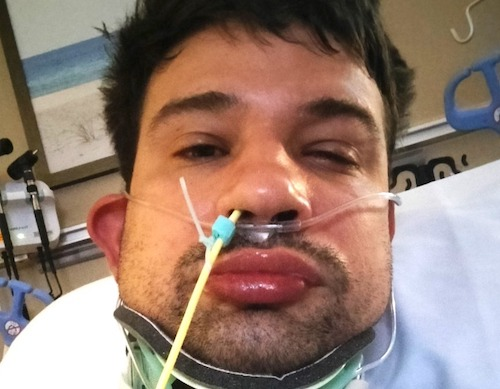
\includegraphics[width=\linewidth]{picture.jpg}
        \end{FlushLeft}
        \justifying
        \large
        \vspace{0.25cm}
        \begin{itemize}
        \item \GetTranslation{Age}: {#3}
        \item \GetTranslation{Injection(s)}: {#4}
        \item \GetTranslation{Dose(s)}: {#5}
        \item \GetTranslation{Adverse Events and Reactions}: {#6}
        \end{itemize}
        \end{minipage}
        \\
        \vspace{0.5cm}
        \justifying
        \setlength{\parindent}{0.25cm}
        #8
        \begin{FlushRight}
          \vspace{0.25cm}
          \qrcode[height=3cm]{#7} \\
          \vspace{0.25cm}
          \href{#7}{#7}
         \end{FlushRight}
         \end{multicols}
       \end{center}
    \vfill
  \end{frame}
}

% \testimony: create a new testimony based on austama template.
%
% @arg1: Firstname Lastname
% @arg2: Location
% @arg3: Age
% @arg4: Vaccine type
% @arg5: Injection dates
% @arg6: Adverse Drug Reaction
% @arg7: Source URL
\newcommand{\testimony}[7]{
  \testimonyWithContent{#1}
                       {#2}
                       {#3}
                       {#4}
                       {#5}
                       {#6}
                       {#7}
                       {\input{content}}
}

% \testimonyNormal: This command is a wrapper around \testimony but with
%                   a text size using \normalsize.
%
% @arg1: Firstname Lastname
% @arg2: Location
% @arg3: Age
% @arg4: Vaccine type
% @arg5: Injection dates
% @arg6: Adverse Drug Reaction
% @arg7: Source URL
\newcommand{\testimonyNormal}[7]{
  \testimonyWithContent{#1}
                       {#2}
                       {#3}
                       {#4}
                       {#5}
                       {#6}
                       {#7}
                       {
                         \normalsize
                         \input{content}
                       }
}

\newenvironment{record}[1]
{
  \newcommand{testimony}[1]{
    #1
  }
}
{}
